\documentclass{book}
\usepackage[a4paper,top=2.5cm,bottom=2.5cm,left=2.5cm,right=2.5cm]{geometry}
\usepackage{makeidx}
\usepackage{natbib}
\usepackage{graphicx}
\usepackage{multicol}
\usepackage{float}
\usepackage{listings}
\usepackage{color}
\usepackage{ifthen}
\usepackage[table]{xcolor}
\usepackage{textcomp}
\usepackage{alltt}
\usepackage{ifpdf}
\ifpdf
\usepackage[pdftex,
            pagebackref=true,
            colorlinks=true,
            linkcolor=blue,
            unicode
           ]{hyperref}
\else
\usepackage[ps2pdf,
            pagebackref=true,
            colorlinks=true,
            linkcolor=blue,
            unicode
           ]{hyperref}
\usepackage{pspicture}
\fi
\usepackage[utf8]{inputenc}
\usepackage{mathptmx}
\usepackage[scaled=.90]{helvet}
\usepackage{courier}
\usepackage{sectsty}
\usepackage{amssymb}
\usepackage[titles]{tocloft}
\usepackage{doxygen}
\lstset{language=C++,inputencoding=utf8,basicstyle=\footnotesize,breaklines=true,breakatwhitespace=true,tabsize=8,numbers=left }
\makeindex
\setcounter{tocdepth}{3}
\renewcommand{\footrulewidth}{0.4pt}
\renewcommand{\familydefault}{\sfdefault}
\hfuzz=15pt
\setlength{\emergencystretch}{15pt}
\hbadness=750
\tolerance=750
\begin{document}
\hypersetup{pageanchor=false,citecolor=blue}
\begin{titlepage}
\vspace*{7cm}
\begin{center}
{\Large Phreeqc-\/\-Fortran \\[1ex]\large ispmarin-\/ulaval-\/01 }\\
\vspace*{1cm}
{\large Generated by Doxygen 1.8.1.2}\\
\vspace*{0.5cm}
{\small Thu Jan 24 2013 12:26:11}\\
\end{center}
\end{titlepage}
\clearemptydoublepage
\pagenumbering{roman}
\tableofcontents
\clearemptydoublepage
\pagenumbering{arabic}
\hypersetup{pageanchor=true,citecolor=blue}
\chapter{Todo List}
\label{todo}
\hypertarget{todo}{}

\begin{DoxyRefList}
\item[\label{todo__todo000003}%
\hypertarget{todo__todo000003}{}%
Subprogram \hyperlink{classbiogeochem_a1bd3b9b68060375fda3f248bc9797483}{biogeochem\-:\-:change\-\_\-components} (id, conc\-\_\-array)]conc\-\_\-array order and sv phreeqc input file must match  
\item[\label{todo__todo000004}%
\hypertarget{todo__todo000004}{}%
Subprogram \hyperlink{classbiogeochem_a3864bdb83fa859558ffd718a003a2e7f}{biogeochem\-:\-:ehandler} (id)]Need to handle other errors  
\item[\label{todo__todo000001}%
\hypertarget{todo__todo000001}{}%
Subprogram \hyperlink{classbiogeochem_ad8fd793d4cfc98786926e183de153627}{biogeochem\-:\-:init\-\_\-phreeq} (id, conc\-\_\-array, input\-\_\-phreeqc\-\_\-file)]
\item[\label{todo__todo000002}%
\hypertarget{todo__todo000002}{}%
Subprogram \hyperlink{classbiogeochem_adb74153c93ecca886574917ee42c6ad4}{biogeochem\-:\-:print\-\_\-components} (id)]
\item[\label{todo__todo000005}%
\hypertarget{todo__todo000005}{}%
Subprogram \hyperlink{classbiogeochem_aed9b27100fe15ac5cfdefac055284e62}{biogeochem\-:\-:run\-\_\-model} (id)]
\item[\label{todo__todo000006}%
\hypertarget{todo__todo000006}{}%
Subprogram \hyperlink{classbiogeochem_add7c48f9d701a9b9a8103e11126fca70}{biogeochem\-:\-:strip\-\_\-header} (id)]
\end{DoxyRefList}
\chapter{Data Type Index}
\section{Data Types List}
Here are the data types with brief descriptions\-:\begin{DoxyCompactList}
\item\contentsline{section}{\hyperlink{classbiogeochem}{biogeochem} \\*Inteface module for Phreeqc and B\-I\-O\-N\-A\-P\-L Ivan Marin -\/ U\-Laval }{\pageref{classbiogeochem}}{}
\end{DoxyCompactList}

\chapter{File Index}
\section{File List}
Here is a list of all files with brief descriptions\-:\begin{DoxyCompactList}
\item\contentsline{section}{/home/ispmarin/src/lavalwork/phreeqc-\/fortran/src/\hyperlink{_i_phreeqc_8f90_8inc}{I\-Phreeqc.\-f90.\-inc} }{\pageref{_i_phreeqc_8f90_8inc}}{}
\item\contentsline{section}{/home/ispmarin/src/lavalwork/phreeqc-\/fortran/src/\hyperlink{phreeqc-fortran_8f90}{phreeqc-\/fortran.\-f90} }{\pageref{phreeqc-fortran_8f90}}{}
\end{DoxyCompactList}

\chapter{Data Type Documentation}
\hypertarget{classbiogeochem}{\section{biogeochem Module Reference}
\label{classbiogeochem}\index{biogeochem@{biogeochem}}
}


Inteface module for Phreeqc and B\-I\-O\-N\-A\-P\-L Ivan Marin -\/ U\-Laval.  


\subsection*{Public Member Functions}
\begin{DoxyCompactItemize}
\item 
subroutine \hyperlink{classbiogeochem_ad8fd793d4cfc98786926e183de153627}{init\-\_\-phreeq} (id, conc\-\_\-array, input\-\_\-phreeqc\-\_\-file)
\begin{DoxyCompactList}\small\item\em Initialization for Phreeqc. \end{DoxyCompactList}\item 
subroutine \hyperlink{classbiogeochem_adb74153c93ecca886574917ee42c6ad4}{print\-\_\-components} (id)
\begin{DoxyCompactList}\small\item\em Print the components of the Solution. \end{DoxyCompactList}\item 
subroutine \hyperlink{classbiogeochem_a1bd3b9b68060375fda3f248bc9797483}{change\-\_\-components} (id, conc\-\_\-array)
\begin{DoxyCompactList}\small\item\em Change the components of the solution from external changes. \end{DoxyCompactList}\item 
subroutine \hyperlink{classbiogeochem_a3864bdb83fa859558ffd718a003a2e7f}{ehandler} (id)
\begin{DoxyCompactList}\small\item\em Call the Error Handler for Phreeqc. \end{DoxyCompactList}\item 
subroutine \hyperlink{classbiogeochem_aed9b27100fe15ac5cfdefac055284e62}{run\-\_\-model} (id)
\begin{DoxyCompactList}\small\item\em Run Phreeqc with id. \end{DoxyCompactList}\item 
subroutine \hyperlink{classbiogeochem_add7c48f9d701a9b9a8103e11126fca70}{strip\-\_\-header} (id)
\begin{DoxyCompactList}\small\item\em Get the name of the components. \end{DoxyCompactList}\item 
integer function \hyperlink{classbiogeochem_afa3f375147a0c61940384264972aa6cb}{strlen} (st)
\end{DoxyCompactItemize}


\subsection{Detailed Description}
Inteface module for Phreeqc and B\-I\-O\-N\-A\-P\-L Ivan Marin -\/ U\-Laval. 

Definition at line 11 of file phreeqc-\/fortran.\-f90.



\subsection{Member Function/\-Subroutine Documentation}
\hypertarget{classbiogeochem_a1bd3b9b68060375fda3f248bc9797483}{\index{biogeochem@{biogeochem}!change\-\_\-components@{change\-\_\-components}}
\index{change\-\_\-components@{change\-\_\-components}!biogeochem@{biogeochem}}
\subsubsection[{change\-\_\-components}]{\setlength{\rightskip}{0pt plus 5cm}subroutine biogeochem\-::change\-\_\-components (
\begin{DoxyParamCaption}
\item[{integer, intent(in)}]{id, }
\item[{character(len=40), dimension(\-:), intent(inout), allocatable}]{conc\-\_\-array}
\end{DoxyParamCaption}
)}}\label{classbiogeochem_a1bd3b9b68060375fda3f248bc9797483}


Change the components of the solution from external changes. 


\begin{DoxyParams}{Parameters}
{\em id} & \\
\hline
{\em conc\-\_\-array} & array of concentrations \\
\hline
\end{DoxyParams}
\begin{DoxyRefDesc}{Todo}
\item[\hyperlink{todo__todo000003}{Todo}]conc\-\_\-array order and sv phreeqc input file must match \end{DoxyRefDesc}


Definition at line 90 of file phreeqc-\/fortran.\-f90.



Here is the call graph for this function\-:\nopagebreak
\begin{figure}[H]
\begin{center}
\leavevmode
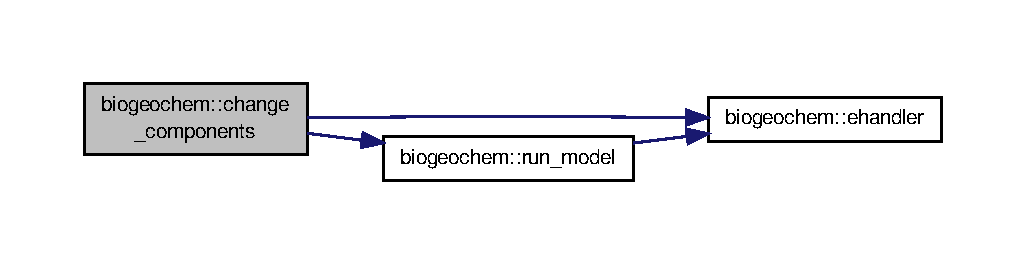
\includegraphics[width=350pt]{classbiogeochem_a1bd3b9b68060375fda3f248bc9797483_cgraph}
\end{center}
\end{figure}




Here is the caller graph for this function\-:\nopagebreak
\begin{figure}[H]
\begin{center}
\leavevmode
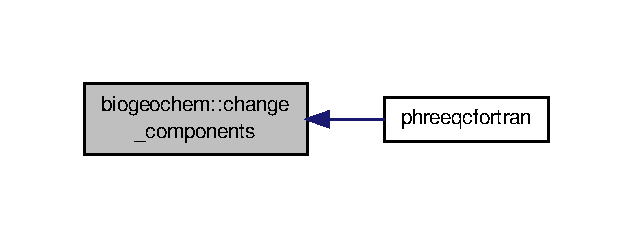
\includegraphics[width=304pt]{classbiogeochem_a1bd3b9b68060375fda3f248bc9797483_icgraph}
\end{center}
\end{figure}


\hypertarget{classbiogeochem_a3864bdb83fa859558ffd718a003a2e7f}{\index{biogeochem@{biogeochem}!ehandler@{ehandler}}
\index{ehandler@{ehandler}!biogeochem@{biogeochem}}
\subsubsection[{ehandler}]{\setlength{\rightskip}{0pt plus 5cm}subroutine biogeochem\-::ehandler (
\begin{DoxyParamCaption}
\item[{integer, intent(in)}]{id}
\end{DoxyParamCaption}
)}}\label{classbiogeochem_a3864bdb83fa859558ffd718a003a2e7f}


Call the Error Handler for Phreeqc. 


\begin{DoxyParams}{Parameters}
{\em id} & \\
\hline
\end{DoxyParams}
\begin{DoxyRefDesc}{Todo}
\item[\hyperlink{todo__todo000004}{Todo}]Need to handle other errors \end{DoxyRefDesc}


Definition at line 137 of file phreeqc-\/fortran.\-f90.



Here is the caller graph for this function\-:\nopagebreak
\begin{figure}[H]
\begin{center}
\leavevmode
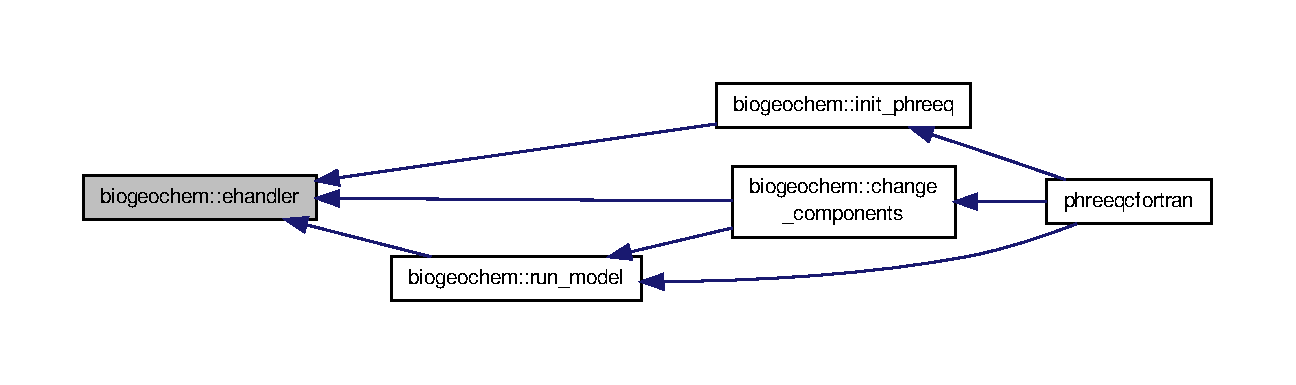
\includegraphics[width=350pt]{classbiogeochem_a3864bdb83fa859558ffd718a003a2e7f_icgraph}
\end{center}
\end{figure}


\hypertarget{classbiogeochem_ad8fd793d4cfc98786926e183de153627}{\index{biogeochem@{biogeochem}!init\-\_\-phreeq@{init\-\_\-phreeq}}
\index{init\-\_\-phreeq@{init\-\_\-phreeq}!biogeochem@{biogeochem}}
\subsubsection[{init\-\_\-phreeq}]{\setlength{\rightskip}{0pt plus 5cm}subroutine biogeochem\-::init\-\_\-phreeq (
\begin{DoxyParamCaption}
\item[{integer, intent(out)}]{id, }
\item[{character(len=40), dimension(\-:), intent(inout), allocatable}]{conc\-\_\-array, }
\item[{character(len=$\ast$), intent(in)}]{input\-\_\-phreeqc\-\_\-file}
\end{DoxyParamCaption}
)}}\label{classbiogeochem_ad8fd793d4cfc98786926e183de153627}


Initialization for Phreeqc. 


\begin{DoxyParams}{Parameters}
{\em id} & \\
\hline
{\em conc\-\_\-array} & \\
\hline
{\em input\-\_\-phreeqc\-\_\-file} & \\
\hline
\end{DoxyParams}
\begin{DoxyRefDesc}{Todo}
\item[\hyperlink{todo__todo000001}{Todo}]\end{DoxyRefDesc}


Definition at line 21 of file phreeqc-\/fortran.\-f90.



Here is the call graph for this function\-:\nopagebreak
\begin{figure}[H]
\begin{center}
\leavevmode
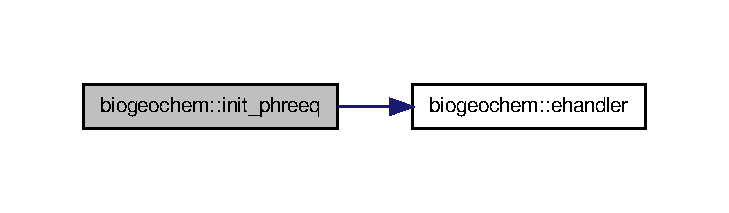
\includegraphics[width=350pt]{classbiogeochem_ad8fd793d4cfc98786926e183de153627_cgraph}
\end{center}
\end{figure}




Here is the caller graph for this function\-:\nopagebreak
\begin{figure}[H]
\begin{center}
\leavevmode
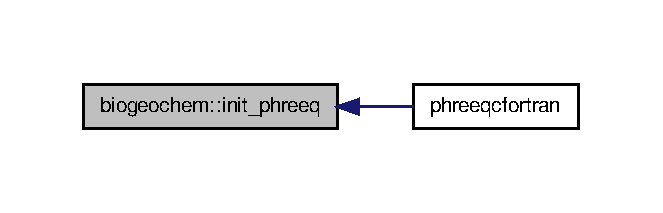
\includegraphics[width=318pt]{classbiogeochem_ad8fd793d4cfc98786926e183de153627_icgraph}
\end{center}
\end{figure}


\hypertarget{classbiogeochem_adb74153c93ecca886574917ee42c6ad4}{\index{biogeochem@{biogeochem}!print\-\_\-components@{print\-\_\-components}}
\index{print\-\_\-components@{print\-\_\-components}!biogeochem@{biogeochem}}
\subsubsection[{print\-\_\-components}]{\setlength{\rightskip}{0pt plus 5cm}subroutine biogeochem\-::print\-\_\-components (
\begin{DoxyParamCaption}
\item[{integer, intent(in)}]{id}
\end{DoxyParamCaption}
)}}\label{classbiogeochem_adb74153c93ecca886574917ee42c6ad4}


Print the components of the Solution. 


\begin{DoxyParams}{Parameters}
{\em id} & \\
\hline
\end{DoxyParams}
\begin{DoxyRefDesc}{Todo}
\item[\hyperlink{todo__todo000002}{Todo}]\end{DoxyRefDesc}


Definition at line 58 of file phreeqc-\/fortran.\-f90.



Here is the caller graph for this function\-:\nopagebreak
\begin{figure}[H]
\begin{center}
\leavevmode
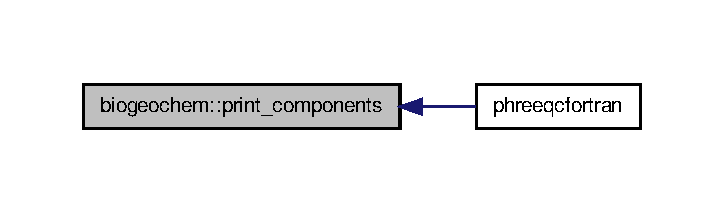
\includegraphics[width=348pt]{classbiogeochem_adb74153c93ecca886574917ee42c6ad4_icgraph}
\end{center}
\end{figure}


\hypertarget{classbiogeochem_aed9b27100fe15ac5cfdefac055284e62}{\index{biogeochem@{biogeochem}!run\-\_\-model@{run\-\_\-model}}
\index{run\-\_\-model@{run\-\_\-model}!biogeochem@{biogeochem}}
\subsubsection[{run\-\_\-model}]{\setlength{\rightskip}{0pt plus 5cm}subroutine biogeochem\-::run\-\_\-model (
\begin{DoxyParamCaption}
\item[{integer, intent(in)}]{id}
\end{DoxyParamCaption}
)}}\label{classbiogeochem_aed9b27100fe15ac5cfdefac055284e62}


Run Phreeqc with id. 


\begin{DoxyParams}{Parameters}
{\em id} & \\
\hline
\end{DoxyParams}
\begin{DoxyRefDesc}{Todo}
\item[\hyperlink{todo__todo000005}{Todo}]\end{DoxyRefDesc}


Definition at line 150 of file phreeqc-\/fortran.\-f90.



Here is the call graph for this function\-:\nopagebreak
\begin{figure}[H]
\begin{center}
\leavevmode
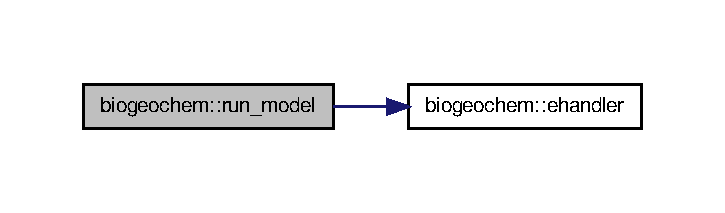
\includegraphics[width=348pt]{classbiogeochem_aed9b27100fe15ac5cfdefac055284e62_cgraph}
\end{center}
\end{figure}




Here is the caller graph for this function\-:\nopagebreak
\begin{figure}[H]
\begin{center}
\leavevmode
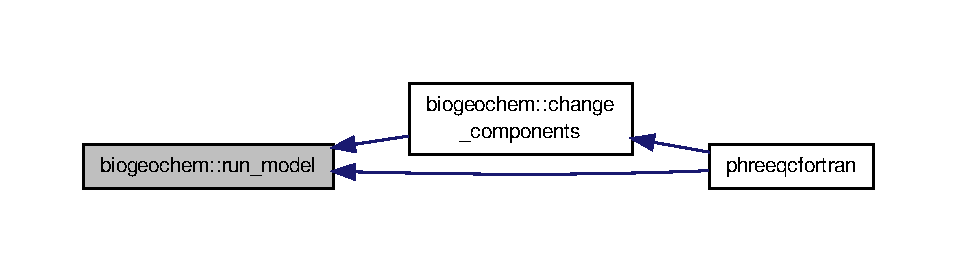
\includegraphics[width=350pt]{classbiogeochem_aed9b27100fe15ac5cfdefac055284e62_icgraph}
\end{center}
\end{figure}


\hypertarget{classbiogeochem_add7c48f9d701a9b9a8103e11126fca70}{\index{biogeochem@{biogeochem}!strip\-\_\-header@{strip\-\_\-header}}
\index{strip\-\_\-header@{strip\-\_\-header}!biogeochem@{biogeochem}}
\subsubsection[{strip\-\_\-header}]{\setlength{\rightskip}{0pt plus 5cm}subroutine biogeochem\-::strip\-\_\-header (
\begin{DoxyParamCaption}
\item[{integer, intent(in)}]{id}
\end{DoxyParamCaption}
)}}\label{classbiogeochem_add7c48f9d701a9b9a8103e11126fca70}


Get the name of the components. 


\begin{DoxyParams}{Parameters}
{\em id} & \\
\hline
\end{DoxyParams}
\begin{DoxyRefDesc}{Todo}
\item[\hyperlink{todo__todo000006}{Todo}]\end{DoxyRefDesc}


Definition at line 164 of file phreeqc-\/fortran.\-f90.

\hypertarget{classbiogeochem_afa3f375147a0c61940384264972aa6cb}{\index{biogeochem@{biogeochem}!strlen@{strlen}}
\index{strlen@{strlen}!biogeochem@{biogeochem}}
\subsubsection[{strlen}]{\setlength{\rightskip}{0pt plus 5cm}integer function biogeochem\-::strlen (
\begin{DoxyParamCaption}
\item[{character, dimension($\ast$)}]{st}
\end{DoxyParamCaption}
)}}\label{classbiogeochem_afa3f375147a0c61940384264972aa6cb}


Definition at line 195 of file phreeqc-\/fortran.\-f90.



The documentation for this module was generated from the following file\-:\begin{DoxyCompactItemize}
\item 
/home/ispmarin/src/lavalwork/phreeqc-\/fortran/src/\hyperlink{phreeqc-fortran_8f90}{phreeqc-\/fortran.\-f90}\end{DoxyCompactItemize}

\chapter{File Documentation}
\hypertarget{_i_phreeqc_8f90_8inc}{\section{/home/ispmarin/src/lavalwork/phreeqc-\/fortran/src/\-I\-Phreeqc.f90.\-inc File Reference}
\label{_i_phreeqc_8f90_8inc}\index{/home/ispmarin/src/lavalwork/phreeqc-\/fortran/src/\-I\-Phreeqc.\-f90.\-inc@{/home/ispmarin/src/lavalwork/phreeqc-\/fortran/src/\-I\-Phreeqc.\-f90.\-inc}}
}

\hypertarget{phreeqc-fortran_8f90}{\section{/home/ispmarin/src/lavalwork/phreeqc-\/fortran/src/phreeqc-\/fortran.f90 File Reference}
\label{phreeqc-fortran_8f90}\index{/home/ispmarin/src/lavalwork/phreeqc-\/fortran/src/phreeqc-\/fortran.\-f90@{/home/ispmarin/src/lavalwork/phreeqc-\/fortran/src/phreeqc-\/fortran.\-f90}}
}
\subsection*{Data Types}
\begin{DoxyCompactItemize}
\item 
module \hyperlink{classbiogeochem}{biogeochem}
\begin{DoxyCompactList}\small\item\em Inteface module for Phreeqc and B\-I\-O\-N\-A\-P\-L Ivan Marin -\/ U\-Laval. \end{DoxyCompactList}\end{DoxyCompactItemize}
\subsection*{Functions/\-Subroutines}
\begin{DoxyCompactItemize}
\item 
program \hyperlink{phreeqc-fortran_8f90_a9714b87ecacd59cf20430f2398694c5f}{phreeqcfortran}
\end{DoxyCompactItemize}


\subsection{Function/\-Subroutine Documentation}
\hypertarget{phreeqc-fortran_8f90_a9714b87ecacd59cf20430f2398694c5f}{\index{phreeqc-\/fortran.\-f90@{phreeqc-\/fortran.\-f90}!phreeqcfortran@{phreeqcfortran}}
\index{phreeqcfortran@{phreeqcfortran}!phreeqc-fortran.f90@{phreeqc-\/fortran.\-f90}}
\subsubsection[{phreeqcfortran}]{\setlength{\rightskip}{0pt plus 5cm}program phreeqcfortran (
\begin{DoxyParamCaption}
{}
\end{DoxyParamCaption}
)}}\label{phreeqc-fortran_8f90_a9714b87ecacd59cf20430f2398694c5f}


Definition at line 209 of file phreeqc-\/fortran.\-f90.



Here is the call graph for this function\-:\nopagebreak
\begin{figure}[H]
\begin{center}
\leavevmode
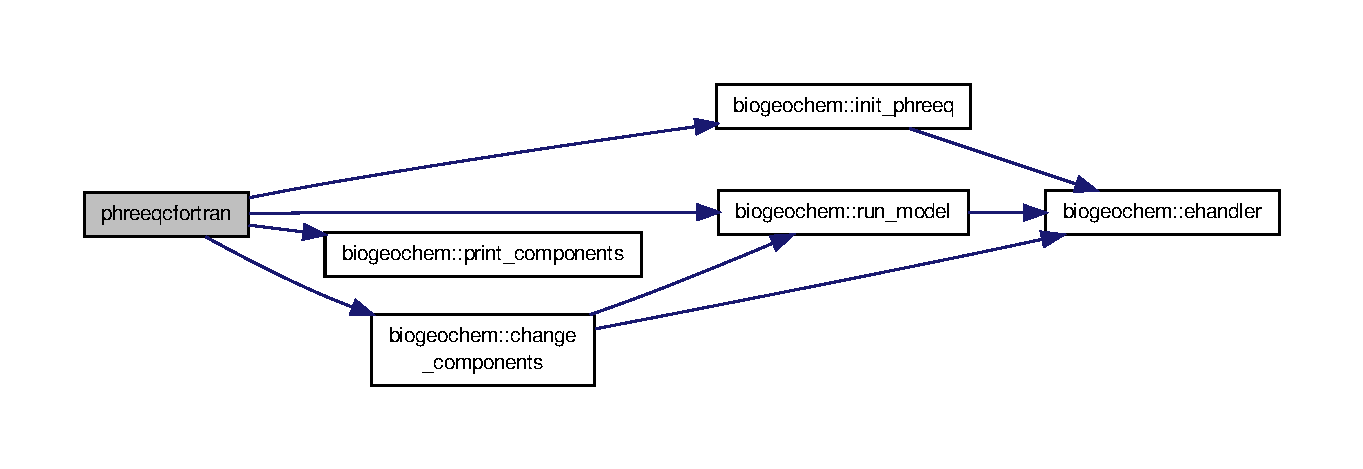
\includegraphics[width=350pt]{phreeqc-fortran_8f90_a9714b87ecacd59cf20430f2398694c5f_cgraph}
\end{center}
\end{figure}



\printindex
\end{document}
